\chapter{Modeling}
\label{sec:modeling}
In this section the MAV overall system which is to be controlled is described. It starts by describing the multirotor platform. Then the equations of motion are derived for both translation and rotation. Additionally we include wind in the model. In the fourth part a system idenfication approach is described to approximate the attitude dynamics. Next the overall dynamics to be controlled are summarized in a system diagram. Finally the system is linearized.

In this project a cascaded control approach is chosen (see figure ). Attitude and motor control run at a high rate ($1000 \si{\hertz}$) in an inner loop, while the high level position controller runs at $100 \si{\hertz}$ in an outer loop. This decoupling is possible because the translational dynamics are much slower than the rotational dynamics. It simplifies the design of the position controller as only translational dynamics have to be considered explicitly and position control reduces to controlling the vehicles desired thrust and direction. 

In order for the vehicle to move to a reference position, the position controller computes the desired thrust force and roll, pitch, yaw angles. The inner loop then takes care of finding the appropriate moment applied to the vehicle body to archieve the desired attitude. The attitude controller is given and its dynamics are identified as a linear system.

\begin{figure}
\centering
\includegraphics{images/controller_sketch.tikz}
\caption{Cascaded control sketch}
\label{pics:controller_sketch}
\end{figure}





Also we only consider translational dynamics as they are crucial for position control. The rotational dynamics are handled by the attitude controller. We approximate the closed loop attitude control with a linear system identification.

%%%%%%%%%%%%%%%%%%%%%%%%%%%%%%%%%%%%%%%%%%%%%%%%%%%%%%%%%%%%%%%%%%%%%%%%%%%%%%%
% Platform
%%%%%%%%%%%%%%%%%%%%%%%%%%%%%%%%%%%%%%%%%%%%%%%%%%%%%%%%%%%%%%%%%%%%%%%%%%%%%%%
\section{Platform}
Within this project we use an AscTec Firefly (see figure \ref{pics:firefly}). While this is a hexacopter, the dynamics and controllers are generalized to fit any multirotor configuration. A multirotor is a flying platform consisting of a body and a user specified arrangement of three or more rotors. Only configurations are considered which have all rotors lying fixed in a plane.

In platforms with even-numbered motors, neighboring rotors typically rotate in opposite direction. This compensates yaw moments and gives control over heading. Tilting is accomplished by increasing the thrust on on one side of the vehicle and decreasing it on the opposite side.

The Firefly has six $8 \si{\in}$ rotors equally aligned around the center. It is $60.5 \times 66.5 \times 16.5 \si{\cm}$ in size and weights $1.6 \si{\kg}$. The maximum thrust is $36 \si{\N}$ and it reaches a maximum airspeed of $15 \si{\metre\per\second}$.

\begin{figure}
   \centering
   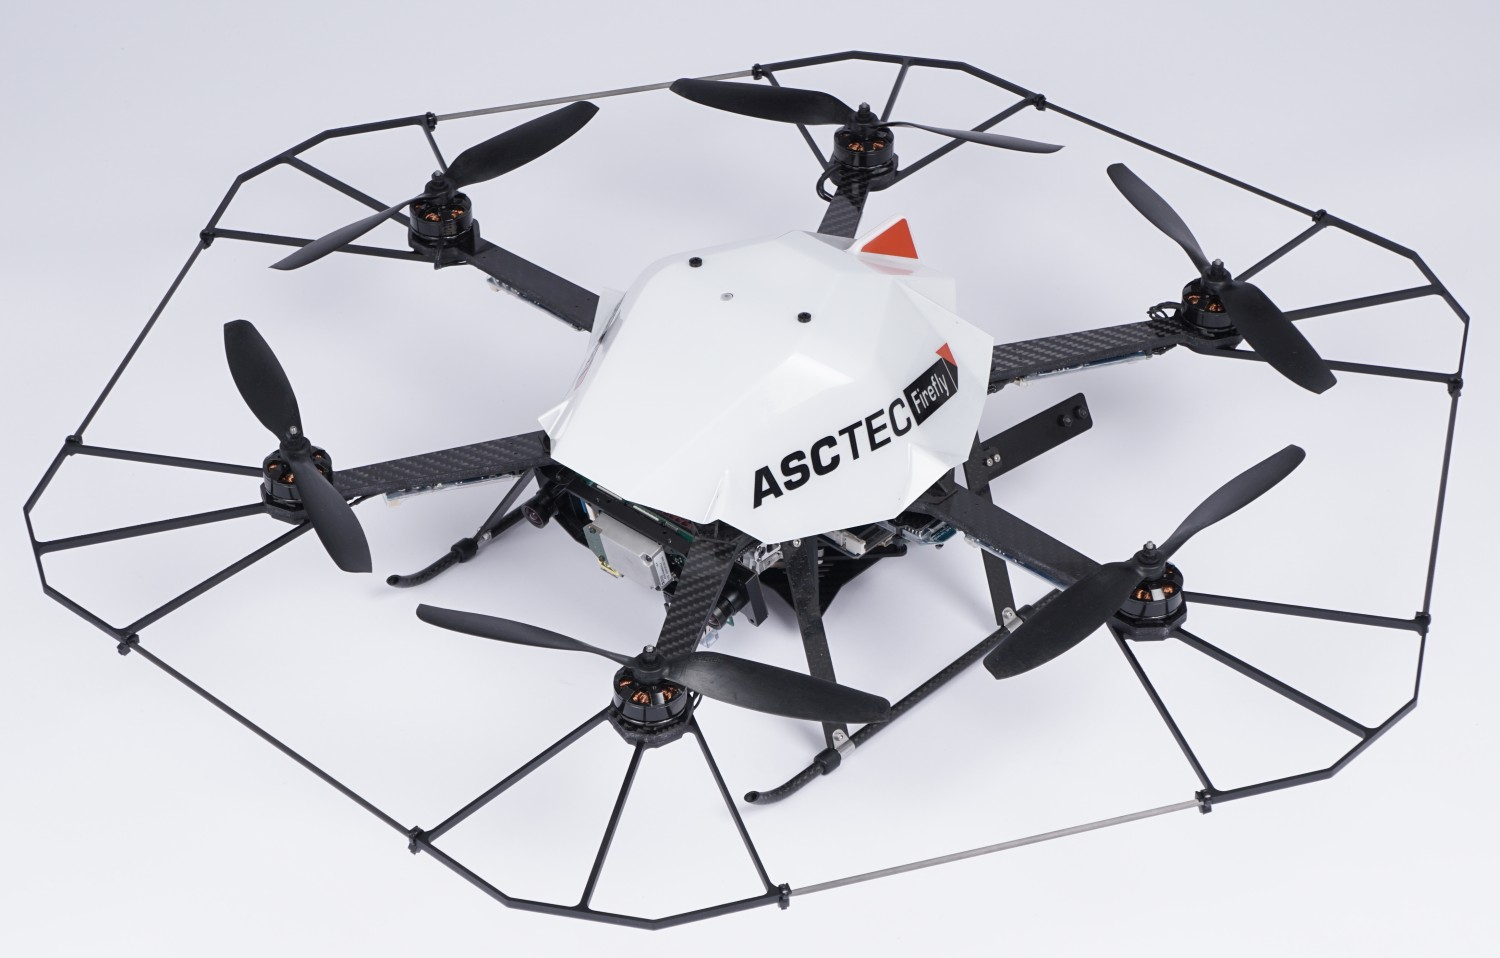
\includegraphics[width=0.75\textwidth]{images/firefly.jpg}
   \caption{AscTec Firefly \cite{www:asctec}}
   \label{pics:firefly}
\end{figure}

It is provided with an inertial measurement unit (IMU) and has a efficient attitude controller onboard. In the experiment an external optical motion capture system by Vicon is used to feedback precise position information. A processor is taking care of online computation.

%%%%%%%%%%%%%%%%%%%%%%%%%%%%%%%%%%%%%%%%%%%%%%%%%%%%%%%%%%%%%%%%%%%%%%%%%%%%%%%
% Equations of Motion
%%%%%%%%%%%%%%%%%%%%%%%%%%%%%%%%%%%%%%%%%%%%%%%%%%%%%%%%%%%%%%%%%%%%%%%%%%%%%%%
\section{Equations of Motion}
The multirotor is modeled as a rigid body with six degrees of freedom (DoF). It has three translational DoF $x$, $y$, $z$ and three rotational DoF roll, pitch and yaw ($\phi$, $\theta$, $\psi$).

 For modeling purposes, we define proper reference frames and notations first. Then the dynamics acting at each rotor are stated. Next the Newton's and Euler's equations for the vehicle are formed giving the complete dynamics of the vehicle.

\subsection{Coordinate Systems and Notations}
In total three main reference frames are defined. The inertial frame $W$, an intermediate heading oriented frame $A$ and a body fixed frame $B$. The inertial frame is world fixed with $z$ pointing upwards collinear to the gravitational force. The heading oriented frame $A$ is produced by rotating the world fixed frame around the $z$-axis through the current heading of the MAV. The body fixed frame is produced by rotating frame $A$ first through the pitch angle about the $y$-axis and then through the roll angle about the $x$-axis. This corresponds to Tait-Bryan angles or $zyx$-sequence. It is located at the body's principal axes of inertia.

We denote vectors and matrices with a bold letter. A leading subscript on a vector denotes the corresponding coordinate frame. A leading double subscript on a matrix denotes the coordinate transformation from the second subscript frame to the first subscript frame. A single trailing subscript serves as additional discriptor. We abbreviate $\sin(\cdot)$ and $\cos(\cdot)$ with $s \cdot$ or $c \cdot$ respectively.

For the rotations we get
\begin{align}
_{BW}\mathbf{R}_x (\phi)&=  \begin{bmatrix}
1 & 0 & 0 \\
0 & c\phi & s\phi \\
0 & -s\phi & c\phi
\end{bmatrix} ,\\
_{BW}\mathbf{R}_y (\theta)&=  \begin{bmatrix}
c\theta & 0 & -s\theta \\
0 & 1 & 0 \\
s\theta & 0 & c\theta
\end{bmatrix} ,\\
_{BW}\mathbf{R}_z (\psi)&=  \begin{bmatrix}
c\psi & s\psi & 0 \\
-s\psi & c\psi & 0 \\
0 & 0 &1
\end{bmatrix}.
\end{align}

Vectors in world frame can then be transformed into body frame and back with
\begin{align}
_{BW}\mathbf{R} (\phi,\theta,\psi) &= {_{BW}\mathbf{R}_x} (\phi) \cdot {_{BW}\mathbf{R}_y} (\theta) \cdot {_{BW}\mathbf{R}_z} (\psi) \\
&=
 \begin{bmatrix}
c\theta c\psi 				&c\theta s\psi 				& -s\theta  \\
s\phi s\theta c\psi - c\phi s\psi  	& s\phi s\theta s\psi + c\phi c\psi 	& s\phi c\theta \\
c\phi s\theta c\psi + s\phi s\psi	& c\phi s\theta s\psi - s\phi c\psi 	& c\phi c\theta
\end{bmatrix} ,\\
_{WB}\mathbf{R} (\phi,\theta,\psi) &= {_{BW}\mathbf{R} (\phi,\theta,\psi)}^{-1} = {_{BW}\mathbf{R} (\phi,\theta,\psi)}^{T} \\
&=
\begin{bmatrix}
c\theta c\psi & s\phi s\theta c\psi - c\phi s\psi & c\phi s\theta c\psi + s\phi s\psi \\
c\theta s\psi & s\phi s\theta s\psi + c\phi c\psi & c\phi s\theta s\psi - s\phi c\psi \\
-s\theta & s\phi c\theta & c\phi c\theta
\end{bmatrix}.
\end{align}

Rotations from the inertial frame to the intermediate heading oriented frame and back are done via
\begin{align}
_{AW}\mathbf{R} (\psi) &= {_{BW}\mathbf{R}_z} (\psi) ,\\
_{WA}\mathbf{R} (\psi) &= {_{AW}\mathbf{R} (\psi)}^{-1} = {_{AW}\mathbf{R} (\psi)}^{T}.
\end{align}

And finally rotations from the intermediate frame to the body frame are
\begin{align}
_{BA}\mathbf{R} (\phi,\theta) &= {_{BW}\mathbf{R}_x} (\phi) \cdot {_{BW}\mathbf{R}_y} (\theta)  ,\\
_{AB}\mathbf{R} (\phi,\theta) &= {_{BA}\mathbf{R} (\phi,\theta)}^{-1} = {_{BA}\mathbf{R} (\phi,\theta)}^{T}.
\end{align}


\subsection{Dynamics}
Martin et al. \cite{Martin2010} propose that the dominant forces and moments acting on a regular multirotor origin from the summation of the aerodynamic effects at each rotor and the gravitational force. We state the rotor dynamics with equations \ref{eq:rotor_begin} to \ref{eq:rotor_begin} which eventually lead to the Newton's equation \ref{eq:newton} and Euler's equation \ref{eq:euler} which completely describe the vehicle equations of motion. We do not model motor dynamics as they are much faster than the translational dynamics.

\subsubsection{Rotor Dynamics}
Blade theory gives the mechanics of each propeller/motor assembly. We neglect 
\begin{itemize} 
\item blade flapping (stiff rotors),
\item high order linear and angular velocity terms (small at hovering compared to blade tip speed),
\item linear and angular acceleration of propellers (low mass),
\item angular acceleration of motors (small at hovering),
\item friction torque due to rotational motion.
\end{itemize}

The remaining major forces are thrust $F_T$ and drag $F_D$. Thrust acts perpendicular to the blade plane and lifts the body. Drag acts opposing to the vehicle's airspeed and slows down the vehicle. The major torques acting on a single blade are roll moments $M_R$ and drag moments $M_D$. The direction of these moments and forces are depicted in figure. 

\begin{align}
\mathbf{F}_T&= \omega^2 \cdot C_T \cdot _B\mathbf{e}_z  &\text{(thrust)} ,\label{eq:rotor_begin} \\
\mathbf{F}_D&= -\omega \cdot  C_D \cdot _B\mathbf{\boldsymbol{\nu}}^\perp  &\text{(drag)} ,\\
\mathbf{M}_R&= \omega \cdot C_R \cdot _B\mathbf{\boldsymbol{\nu}}^\perp &\text{(roll)} , \\
\mathbf{M}_D&= -\epsilon \cdot C_M \cdot \mathbf{F_T}  &\text{(drag)}, \label{eq:rotor_end}
\end{align}
where
\begin{align*}
\omega &: &\text{angular velocity of rotor blade}, \\
C_T>0 &: &\text{thrust constant}, \\
C_D>0 &: &\text{drag constant}, \\
C_R>0 &: &\text{rolling moment constant}, \\
C_M>0 &: &\text{drag moment constant}, \\
\epsilon\in\{-1,1\} &: &\text{turning direction (clockwise, counter clockwise)}, \\
_B\mathbf{e}_z &: &\text{unit vector in z-direction in base coordinates},\\
_B\mathbf{\boldsymbol{\nu}} &: &\text{airspeed in base coordinates} .
\end{align*}

The $\perp$-symbol denotes the projection of the air speed on the propeller plane (see figure). It can be calculated as:

\begin{align}
_B\mathbf{\boldsymbol{\nu}}^\perp = _B\mathbf{e}_z \times (_B\mathbf{\boldsymbol{\nu}} \times _B\mathbf{e}_z) = _B\mathbf{\boldsymbol{\nu}} - ( _B\mathbf{\boldsymbol{\nu}} \cdot _B\mathbf{e}_z) \cdot _B\mathbf{e}_z .
\end{align}

\subsubsection{Newton's Equations}
The acceleration $\mathbf{a}$ in world frame can be found using Newton's second law. The sum of all forces acting induced by the $n$ rotors and the gravitational force $\mathbf{F}_G$ equals to the body mass $m$ multiplied with the body acceleration.
\begin{align}
\mathbf{F} = m \cdot \mathbf{a} = _{WB}\mathbf{R} \sum_{i=1}^n \underbrace{\left(\mathbf{F}_{T,i} + \mathbf{F}_{D,i} \right)}_{=:\mathbf{F}_i} + \mathbf{F}_G \label{eq:newton}
\end{align}

\subsubsection{Euler's Equations}
The torque $\boldsymbol{\tau}$ acting on vehicle body's base can be found using Euler's equations for rigid body dynamics.  
\begin{align}
\boldsymbol{\tau} = \mathbf{J} \cdot  \mathbf{\dot{\boldsymbol{\omega}}} + \boldsymbol{\omega} \times \mathbf{J} \cdot \boldsymbol{\omega} = \sum_{i=1}^n \left( \mathbf{M}_{R,i}+ \mathbf{M}_{D,i} + \mathbf{F}_i \times \mathbf{r}_i \right)  \label{eq:euler}
\end{align}
$\mathbf{J}$  is the inertia matrix referenced to the center of mass along the base frame. $\boldsymbol{\omega}$ is the angular velocity about the same frame. $\mathbf{r}_i$ denotes the vector from the CoG of the MAV to the $i$-th rotor.

The moment equations are dispensible, because attitude control is taken care of by an implemented controller already. We still write them down for completeness.

%%%%%%%%%%%%%%%%%%%%%%%%%%%%%%%%%%%%%%%%%%%%%%%%%%%%%%%%%%%%%%%%%%%%%%%%%%%%%%%
% System Formulation
%%%%%%%%%%%%%%%%%%%%%%%%%%%%%%%%%%%%%%%%%%%%%%%%%%%%%%%%%%%%%%%%%%%%%%%%%%%%%%%
\section{System Formulation}
